\documentclass{article}

\usepackage[utf8]{inputenc}
\usepackage[nottoc]{tocbibind}
\usepackage[dvipsnames]{xcolor}
\usepackage[labelfont=bf]{caption}
\usepackage[left=20mm, top=15mm, right=15mm, bottom=15mm, nohead, footskip=10mm]{geometry}

\usepackage{tikz}
\usepackage{lscape}
\usepackage{amsthm}
\usepackage{amssymb}
\usepackage{amsmath}
\usepackage{comment}
\usepackage{hyperref}
\usepackage{graphicx}
\usepackage{hyperref}
\usepackage{booktabs}
\usepackage{listings}
\usepackage{pythontex} 
\usepackage{adjustbox}
\usepackage{subcaption}

% \lstset{basicstyle=\small\ttfamily}

% \lstset{language=Python}
% \lstset{frame=lines}
% % \lstset{caption={Insert code directly in your document}}
% \lstset{label={lst:code_direct}}
% \lstset{basicstyle=\footnotesize}

\hypersetup{
    colorlinks=true,
    linkcolor=blue,    
    urlcolor=blue,
    citecolor=blue
}

\definecolor{codegreen}{rgb}{0,0.6,0}
\definecolor{codegray}{rgb}{0.5,0.5,0.5}
\definecolor{codepurple}{rgb}{0.58,0,0.82}
\definecolor{backcolour}{rgb}{0.95,0.95,0.92}

\lstdefinestyle{mystyle}{
    backgroundcolor=\color{backcolour},   
    commentstyle=\color{codegreen},
    keywordstyle=\color{magenta},
    numberstyle=\tiny\color{codegray},
    stringstyle=\color{codepurple},
    basicstyle=\ttfamily\footnotesize,
    breakatwhitespace=false,         
    breaklines=true,                 
    captionpos=b,                    
    keepspaces=true,                 
    numbers=left,                    
    numbersep=5pt,                  
    showspaces=false,                
    showstringspaces=false,
    showtabs=false,                  
    tabsize=2
}

\lstset{style=mystyle}

\DeclareMathOperator{\dif}{d}
\DeclareMathOperator{\Cov}{Cov}
\DeclareMathOperator{\E}{\mathbb{E}}

\renewcommand{\P}{\mathbb{P}}

\title{Networks II \\ Project I Report}
\author{Bulat Khamitov}
\date{September 15, 2020}

\linespread{1.5}

\begin{document}

\maketitle

\tableofcontents

\section{Task Description}

Solve the \href{http://vladowiki.fmf.uni-lj.si/doku.php?id=ru:hse:snet:problems}{problem} with your \href{http://vladowiki.fmf.uni-lj.si/doku.php?id=ru:hse:snet19:students}{number} with the Monte Carlo method. 
If you are able to solve it also theoretically, compare both results.

\subsection*{Problem 9}

A convex shape $L$ is given.
What is the probability that the randomly selected four points in $L$ will determine a convex quadrilateral? 
Solve for $L$ being an equilateral triangle. 
\href{http://vladowiki.fmf.uni-lj.si/doku.php?id=ru:hse:snet:problems#hint_1}{[Hint 1]}.

\newpage

\section{Analytical Solution}

\subsection{Sylvester's Four Point Problem}

The problem proposed for a student to solve, in its general form represents nothing but \textit{Sylvester's four point problem} \cite{sylvester}.
The solution below is based on paragraph 2.2.6 from \cite{geom}.

We consider a convex domain $L$.
We assume that four points are selected independently and randomly inside $L$.
The probability is proportional to the area of $L$.
What is the probability that these four points form a convex quadrilateral?

Without any loss of generality, we suppose that $3$ points do not fall on one the same line.
These $3$ points form a triangle.
If the $4$-th point falls inside this triangle, then the $4$ points form not a convex quadrilateral, but a re-entrant one (non-convex).
\begin{figure}[ht]
    \centering
    \begin{minipage}[b]{0.2\textwidth}
        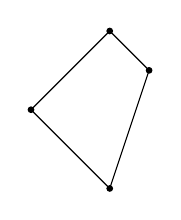
\begin{tikzpicture}
            \draw[black] (1.0, 1.5) -- (2.0, 0.5) -- (2.5, 2.0) -- (2.0, 2.5) -- cycle;
            \filldraw[black] (1.0, 1.5) circle (1pt);
            \filldraw[black] (2.0, 0.5) circle (1pt);
            \filldraw[black] (2.5, 2.0) circle (1pt);
            \filldraw[black] (2.0, 2.5) circle (1pt);
        \end{tikzpicture}        
    \end{minipage}
    \begin{minipage}[b]{0.1\textwidth}
        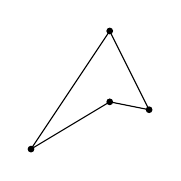
\begin{tikzpicture}
            \draw[black] (1.0, 1.5) -- (2.0, 2.1) -- (2.5, 2.0) -- (2.0, 3.0) -- cycle;
            \filldraw[black] (1.0, 1.5) circle (1pt);
            \filldraw[black] (2.0, 2.1) circle (1pt);
            \filldraw[black] (2.5, 2.0) circle (1pt);
            \filldraw[black] (2.0, 3.0) circle (1pt);
        \end{tikzpicture}       
    \end{minipage}
    \caption{Convex and re-entrant quadrilaterals.}
\end{figure}
The three points forming the triangle or the fourth point can be selected in
\begin{equation*}
    \binom{4}{3} = \binom{4}{1} = 4
\end{equation*}
ways.
Let $X$, $Y$ and $Z$ be the three points.
Then the probability $p$ of the four points forming a re-entrant quadrilateral is given by
\begin{equation*}
    \begin{aligned}
        p &= 4\left[\frac{\text{expexted area of the triangle }XYZ}{\text{area of the convex figure } L}\right] 
        \\
        &= \frac{4}{S}\E[\text{area of } XYZ],
    \end{aligned}
\end{equation*}
where $\E$ denotes the expected value and $S$ is the area of $L$.
Then
\begin{equation*}
    p^{*} = 1 - p
\end{equation*}
is the probability of the four points forming a convex quadrilateral.

Let $p_{1}$ be the same probability as $p$ when one of the three points is on the boundary of $L$.
From Crofton's theorem on measures \cite{geom} we have
\begin{equation*}
    \dif f = \frac{4}{S}[p_{1} - p]\dif S.
\end{equation*}
Let $Z$ be the point on the boundary.
This means that $X$ and $Y$ are independently chosen inside $L$ and $Z$ is uniformly distributed over the perimeter of $L$.

Let the triangle $T$ be $ABC$.
\begin{figure}[h!]
    \centering
    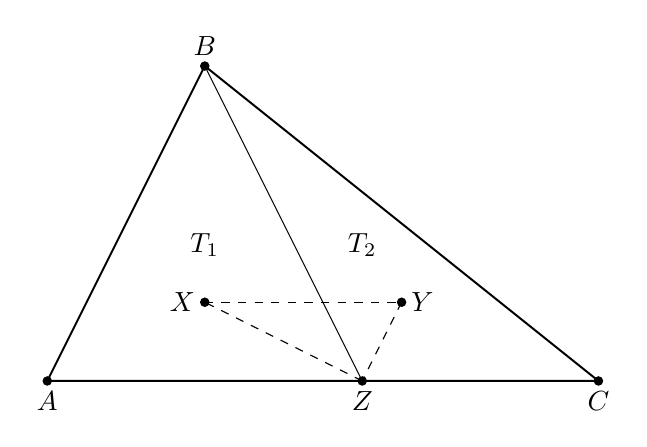
\begin{tikzpicture}
        \draw[line width=0.25mm] (0.0, 0.0) node[anchor=north]{$A$} -- (2.0, 4.0) node[anchor=south]{$B$} -- (7.0, 0.0) node[anchor=north]{$C$} -- (4.0, 0.0) node[anchor=north]{$Z$} -- (0.0, 0.0);

        \draw (2.0, 4.0) -- (4.0, 0.0);

        \draw[dashed] (2.0, 1.0) -- (4.5, 1.0);
        \draw[dashed] (4.5, 1.0) -- (4.0, 0.0);
        \draw[dashed] (4.0, 0.0) -- (2.0, 1.0);

        \filldraw[black] (2.0, 1.0) node[anchor=east]{$X$} circle (1.5pt);
        \filldraw[black] (4.5, 1.0) node[anchor=west]{$Y$} circle (1.5pt);

        \draw (2.0, 2.0) node[anchor=north]{$T_{1}$};
        \draw (4.0, 2.0) node[anchor=north]{$T_{2}$};

        \filldraw[black] (0.0, 0.0) circle (1.5pt);
        \filldraw[black] (2.0, 4.0) circle (1.5pt);
        \filldraw[black] (7.0, 0.0) circle (1.5pt);
        \filldraw[black] (4.0, 0.0) circle (1.5pt);
    \end{tikzpicture}
    \caption{$2$ random points inside a triangle.}
\end{figure}
Let the point $Z$ be on the side $BC$.
Let $T_{1}$ and $T_{2}$ denote the triangles $ABZ$ and $AZC$ respectively.
Let $X$ and $Y$ be the random points within $T$.
There are $4$ possible cases:
\begin{itemize}
    \item $X, Y \in T_{1}$;
    \item $X, Y \in T_{2}$;
    \item $X\in T_{1}$, $Y\in T_{2}$;
    \item $X\in T_{2}$, $Y\in T_{1}$.
\end{itemize}
Since $Z$ is fixed on $BC$, by $\E_{z}(\text{area of }XYZ)$ we denote the expected value of the area of $XYZ$.
Then we have
\begin{equation*}
    \begin{split}
        \E_{z}(\text{area of }XYZ) &= \E_{z}(\text{area of }XYZ\mid X, Y \in T_{1})\P(X\in T_{1})\P(Y\in T_{1})
        \\
        &+ \E_{z}(\text{area of }XYZ\mid X, Y \in T_{2})\P(X\in T_{2})\P(Y\in T_{2})
        \\
        &+ \E_{z}(\text{area of }XYZ\mid X \in T_{1}, Y \in T_{2})\P(X\in T_{1})\P(Y\in T_{2})
        \\
        &+ \E_{z}(\text{area of }XYZ\mid X \in T_{2}, Y \in T_{1})\P(X\in T_{2})\P(Y\in T_{1}),
    \end{split}
\end{equation*}
where $\P(\cdot)$ denotes the probability of the event $(\cdot)$.
Then we have
\begin{equation*}
    \begin{split}
        \E_{z}(\text{area of } XYZ) &= \E_{z}(\text{area of }XYZ\mid X, Y\in T_{1})\frac{S_{1}^{2}}{S^{2}}
        \\
        &+ \E_{z}(\text{area of }XYZ\mid X, Y\in T_{2})\frac{S_{2}^{2}}{S^{2}}
        \\
        &+ 2\E_{z}(\text{area of }XYZ\mid X\in T_{1},Y\in T_{2})\frac{S_{1}S_{2}}{S^{2}},
    \end{split}
\end{equation*}
where $S_{1}$, $S_{2}$ and $S$ are the areas of the triangles $T_{1}$, $T_{2}$ and $T$.
After several steps, we get the following:
\begin{equation*}
    \begin{split}
        \E_{z}(\text{area of }XYZ\mid X\in T_{1}, Y\in T_{2}) &= \frac{1}{9}S,
        \\
        \E_{z}(\text{area of }XYZ\mid X, Y\in T_{1}) &= \frac{4}{27}S_{1},
        \\
        \E_{z}(\text{area of }XYZ\mid X, Y\in T_{2}) &= \frac{4}{27}S_{2}.
    \end{split}
\end{equation*}
We get for $X$, $Y$ belonging to the triangle $T = ABC$ and $Z$ a fixed point on the boundary
\begin{equation*}
    \E(\text{area of } XYZ\mid X, Y, Z \in T) = \frac{1}{S^{2}}\left\{\frac{4}{27}S_{1}^{3} + \frac{4}{27}S_{2}^{3} + \frac{2}{9}SS_{1}S_{2}\right\}.
\end{equation*}
Then from the area of the triangle $T$ is
\begin{equation*}
    S = \frac{1}{2}ah_{1} = \frac{1}{2}bh_{2} = \frac{1}{2}ch_{3}.
\end{equation*}

Since $S_{2} = S - S_{1}$, we write
\begin{equation*}
    \frac{1}{S^{2}}\left\{\frac{4}{27}S_{1}^{3} + \frac{4}{27}S_{2}^{3} + \frac{2}{9}SS_{1}S_{2}\right\} = \frac{4}{27}S - \frac{2}{9}S_{1} + \frac{2}{9}\frac{S_{1}^{2}}{S}.
\end{equation*}

Let $a + b + c = \delta$ and let $Z$ be uniformly distributed over $[0,\,\delta]$.

\begin{equation*}
    \begin{split}
        S_{1} &= \frac{xh_{1}}{2},\quad 0 \leqslant x \leqslant a 
        \\
        &= (x - a)\frac{h_{2}}{2},\quad a \leqslant x \leqslant a + b
        \\
        &= (x - a - b)\frac{h_{3}}{2},\quad a + b \leqslant x \leqslant a + b + c = \delta.
    \end{split}
\end{equation*}
Then,
\begin{equation*}
    \begin{split}
        -\frac{2}{9}\int S_{1}\frac{\dif x}{\delta} &= -\frac{2}{9}\Bigg\{\frac{h_{1}}{2}\int_{0}^{a}x\dif x + \frac{h}{2}\int_{a}^{a + b}(x - a)\dif x + \frac{h_{3}}{2}\int_{a + b}^{a + b + c}(x - a - b)\dif x\Bigg\}
        \\
        &= -\frac{2}{9\delta}\left\{\frac{h_{1}^{2}}{4}a^{2} + \frac{h_{2}^{2}}{4}b^{2} + \frac{h_{3}^{2}}{4}c^{2}\right\}.
    \end{split}
\end{equation*}
\begin{equation*}
    \frac{2}{9}\int S_{1}^{2}\frac{\dif x}{\delta} = \frac{2}{9S\delta}\left\{\frac{h_{1}^{2}}{12}a^{3} + \frac{h_{2}^{2}}{12}b^{3} + \frac{h_{3}^{2}}{12}c^{3}\right\} = \frac{2}{9\delta}\left\{\frac{h_{1}a^{2}}{6} + \frac{h_{2}b^{2}}{6} + \frac{h_{3}c^{2}}{6}\right\}.
\end{equation*}
Hence,
\begin{equation*}
    -\frac{2}{9}\int S_{1}\frac{\dif x}{\delta} + \frac{2}{9S}\int S_{1}^{2}\frac{\dif x}{\delta} = -\frac{1}{54}(h_{1}a^{2} + h_{2}b^{2} + h_{3}c^{2}) = -\frac{S}{27\delta}(a + b + c) = -\frac{S}{27}.
\end{equation*}
Then from the unconditional expectation of the area $XYZ$ when $Z$ is on the boundary of the triangle is
\begin{equation*}
    \frac{4}{27}S - \frac{S}{27} = \frac{1}{9}S.
\end{equation*}
There are $3$ possibilities of $Z$ or $X$ or $Y$ being on the boundary.
Hence, the unconditional expectation of the area $XYZ$ when any one of the $3$ points is on the boundary of the triangle is
\begin{equation*}
    \frac{3}{9}S = \frac{1}{3}S \rightarrow p_{1} = \frac{1}{3}.
\end{equation*}

\begin{equation*}
    \dif p = \frac{4}{S}(p_{1} - p)\dif S \rightarrow \frac{\dif}{\dif S}(S^{4}p) = 4S^{3}p_{1} = \frac{4}{3}S^{3}.
\end{equation*}
That is, $S^{4}p = \tfrac{S^{4}}{3} + c$, where $c = 0$, giving
\begin{equation*}
    p = \frac{1}{3}.
\end{equation*}
% Thus, in general, when $p$ does not depend on the area or a shape of the convex figure, we need to compute only $p_{1}$ ($p_{1} = p$).
Hence,
\begin{equation*}
    p^{*} =  1 - p = 1 - \frac{1}{3} = \frac{2}{3}.
\end{equation*}

\subsection{Combinatorial Approach}

Another generalization asks the probability that $n$ randomly selected points in a fixed convex domain $L\in\mathbb{R}^{2}$ are the vertices of a convex $n$-gon.
The solution is
\begin{equation*}
    P_{n} = \frac{2^{n}(3n - 3)!}{[(n - 1)!]^{3}(2n)!}
\end{equation*}
for a triangular domain \cite{valtr}.
Having $n = 4$ points would give us
\begin{equation*}
    P_{4} = \frac{2^{4}(12 - 3)!}{[3!]^{3}8!} = \frac{144}{216} = \frac{2}{3}.
\end{equation*}

\newpage 

\section{Monte-Carlo Simulation}

\subsection{Triangle Point Picking}
For a triangle with vertices $(A, B, C)$, we construct a point on its surface by generating two random numbers, $r_1$ and $r_2$, between $0$ and $1$, and evaluating the following equation \cite{shape}:
\begin{equation*}
    P = (1 - \sqrt{r_{1}})A + \sqrt{r_{1}}(1 - r_{2})B + \sqrt{r_{1}}r_{2}C.
\end{equation*}
Intuitively, $\sqrt{r_{1}}$ sets the percentage from vertex $A$ to the opposing edge, while $r_{2}$ represents the percentage along that edge. 
Taking the $\sqrt{r_{1}}$ gives a uniform random point with respect to surface area.

\begin{lstlisting}[language=Python, caption=Sampling a point inside a triangle.]
    import random

    def tri_sample(A, B, C):
        r1 = random.random()
        r2 = random.random()
    
        s1 = math.sqrt(r1)
    
        x = A[0] * (1.0 - s1) + B[0] * (1.0 - r2) * s1 + C[0] * r2 * s1
        y = A[1] * (1.0 - s1) + B[1] * (1.0 - r2) * s1 + C[1] * r2 * s1
    
        return (x, y)    
\end{lstlisting}

For simplicity, we consider a unit triangle.
Hence, the vertices $A$, $B$ and $C$ have the following coordinates:
\begin{equation*}
    A = (0.0,\, 0.0),\quad B = \left(0.5,\, \frac{\sqrt{3}}{2}\right),\quad C = (1.0,\, 0.0).
\end{equation*}

\begin{figure}[ht!]
    \centering
    \begin{minipage}[t]{0.4\textwidth}
        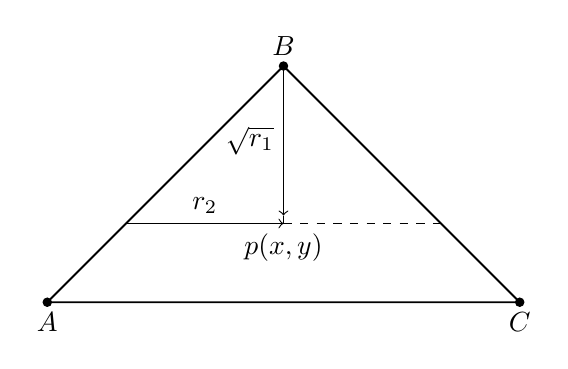
\begin{tikzpicture}
            \draw[line width=0.25mm] (0.0, 0.0) node[anchor=north]{$A$} -- (3.0, 3.0) node[anchor=south]{$B$} -- (6.0, 0.0) node[anchor=north]{$C$} -- cycle;
            
            \draw[->] (3.0, 3.0) -- node[left] {$\sqrt{r_{1}}$} (3.0, 1.1);
            \draw[->] (1.0, 1.0) -- node[midway, above] {$r_{2}$} (3.0, 1.0);
    
            \draw [dashed] (3.0, 1.0) -- (5.0, 1.0);
            \draw [dashed] (3.0, 1.1) -- (3.0, 1.0);
    
            \filldraw[black] (0.0, 0.0) circle (1.5pt);
            \filldraw[black] (3.0, 3.0) circle (1.5pt);
            \filldraw[black] (6.0, 0.0) circle (1.5pt);
            
            \draw (3.0, 1.0) node[anchor=north]{$p(x, y)$};
        \end{tikzpicture}
        \subcaption{Sampling a random point in a triangle.}
    \end{minipage}
    \begin{minipage}[t]{0.4\textwidth}
        \includegraphics[scale=0.3]{images/equilateral_triangle.pdf}
        \subcaption{Equilateral triangle with $N = 10000$ points.}
    \end{minipage}    
    %\caption{test.}
\end{figure}

\newpage

\subsection{Quadrilateral Check}

For any triple points of $A$, $B$ and $C$ in the plane, we can determine whether the angle $A-B-C$ makes a counterclockwise or a clockwise turn.
We call $4$ points and compute these signs for each of the four triples.
If all signs are equal or there are $2$ positive and $2$ negative signs, the convex hull is a quadrilateral.
If there are $3$ positive and $1$ negative sign, the convex hull is a triangle.

We assume that no $3$ points are collinear.

\begin{lstlisting}[language=Python, caption=Sign definition function.]
    def sign(x):
    """ Return the sign of a finite number x. """
        if x > 0:
            return 1
        elif x < 0:
            return -1
        else:
            return 0    
\end{lstlisting}

\begin{lstlisting}[language=Python, caption=Turn definition function.]
    def ccw(A, B, C):
    """ Return 1 if A-B-C is a counterclockwise turn, 
              -1 for clockwise,
               0 if the points are collinear (or not all distinct). """
        disc = (A[0] - C[0]) * (B[1] - C[1]) - (A[1] - C[1]) * (B[0] - C[0])
        return sign(disc)
\end{lstlisting}

Then goes the classification of a quadruple of points:
\begin{lstlisting}[language=Python, caption=Point classification function.]
    def classify_points(A, B, C, D):
    """ Return 1 if a convex hull of A, B, C and D is a quadrilateral,
              -1 if a triangle,
               0 if any three of A, B, C and D are collinear (or if not all points are distinct). """
        return ccw(A, B, C) * ccw(A, B, D) * ccw(A, C, D) * ccw(B, C, D)
\end{lstlisting}

\newpage

\subsection{Monte-Carlo Method}

Classical definition of probability:
\begin{equation*}
    \P = \frac{\text{number of favorable outcomes}}{\text{total number of possible outcomes}}.
\end{equation*}
In our case, favorable outcome would be each time a convex quadrilateral is formed.
The procedure is quite simple:
\begin{enumerate}
    \item On a given triangle domain pick 4 random points;
    \item Check if they form a convex quadrilateral;
    \item If they do, increase a special counter per $1$;
    \item Repeat previous steps $10.000$ times;
    \item Using the above classical definition of probability, compute the chances of forming a convex quadrilateral.
\end{enumerate}

\section{Comparison of Results}
\begin{figure}[h!]
    \centering
    \includegraphics[width=1.0\textwidth]{images/result.pdf}
    \caption{Monte-Carlo simulation compared to the analytical solution.}
\end{figure}

As we can see, the simulation results tend to match the theoretical one, when the number of choices approaches $10.000$.

\newpage

\begin{thebibliography}{9}
    \bibitem{sylvester} 
    Sylvester, J. J., Problem 1491,
    \textit{The Educational Times},
    London, (April, 1864).

    \bibitem{geom}
    Mathai, A. M., An Introduction to Geometrical Probability: Distributional Aspects with Applications (Statistical Distributions \& Models with Applications),
    \textit{CRC Press},
    Australia, (December, 1999).

    \bibitem{valtr}
    Valtr, P., The Probability that $n$ Random Points in a Triangle are in Convex Position,
    \textit{Combinatorica 16},
    (567-573, 1996).

    \bibitem{shape}
    Osada, R., Funkhouser, T., Chazelle, B., and Dobkin, D. Shape Distributions,
    \textit{Association for Computing Machinery},
    New York, USA, (October 2002).
\end{thebibliography}
\end{document}
